\documentclass[lithuanian,a4paper,12pt]{article}
\usepackage{babel}
\babelfont{rm}{FreeSerif}
% \usepackage[T1]{fontenc} % Don't need this when using LuaLatex instead of PDFLatex
\usepackage{amsmath}
\usepackage{graphicx}
\usepackage{float}
\usepackage{listings}
\usepackage{xcolor}

\title{Vienmatis optimizavimas}
\author{Kristupas Dansevičius}
\date{\today}

\begin{document}
\maketitle
\tableofcontents

\section{Įvadas}
Šis laboratorinis darbas atsiskaitomas optimizavimo metodų kurse Vilniaus Universitete. 
Šiame darbe nagrinėjami trys vienmačio optimizavimo metodai:
intervalo dalijimo pusiau metodas, auksinio pjūvio metodas ir Niutono metodas. 

\section{Užduotis}
1-ojo laboratorinio darbo (iš viso yra 4 per semestrą) užduoties reikalavimai:
\begin{enumerate}
    \item Suprogramuoti šiuos metodus (naudota Python programavimo kalba)
    \item Aprašyti duotąją \textbf{tikslo funkciją} - tai funkcija, pagal kurią yra optimizuojama naudojant minėtus metodus, t.y., ieškomas jos \textbf{lokalus minimumas}, kuris ir bus ir \textbf{globalusis minimumas}. Taip yra todėl, kad funkcija yra \textbf{iškiloji}: tarp bet kurių dviejų funkcijos taškų nubrėžus liniją, visos funkcijos reikšmės yra žemiau šios linijos. Kitaip pasakius, funkcijoje nėra jokių "duobių", į kurias optimizuojant galima patekti ir "užstrigti", kurios būtų tik lokalūs, bet ne globalūs minimumai.  
        \begin{equation}
            f(x) = \frac{(x^2 - 5)^2}{4}
        \end{equation}
    \item Minimizuoti funkciją intervalo metodais - intervalo dalijimo pusiau ir auksinio pjūvio - naudojant intervalą $[0,10]$ iki tikslumo $10^{-4}$ bei Niutono metodu nuo $x_0 = 5$ kol žingsnio ilgis (Lipschitzo konstanta / tolerancija) didesnis už $10^{-4}$
    \item Palyginti rezultatus: gauti sprendiniai, rastas funkcijos minimumo įvertis (taško, kuriame funkcija turi mažiausią reikšmę), atliktų žingsnių (iteracijų) ir funkcijų skaičiavimų skaičius (tikslo funkcijos "iškvietimų" programoje)
    \item Vizualizuoti tikslo funkciją ir bandymo taškus (kuriuose paskaičiuota tikslo funkcija ir buvo naudojami algoritme)
\end{enumerate}

\section{Tikslo funkcijos aprašymas}


\section{Metodai}
\subsection{Intervalo dalijimo pusiau metodas}
Tai tritaškis intervalo dalijimo pusiau metodas (t.y., kiekvienai optimizavimo algoritmo iteracijai naudojami 3 taškai), kurio principas yra itin paprastas. Intervale panaudojami 3 taškai:
\begin{itemize}
    \item $x_{middle}$ - tai vidurinis taškas esantis intervalo viduryje
    \item $x_1$ - tai viduryje tarp kairiojo intervalo krašto ir vidurinio taško $x_{middle}$ esantis taškas
    \item 
\end{itemize}

\subsection{Auksinio pjūvio metodas}
Trumpas metodo aprašymas.

\subsection{Niutono metodas}
Trumpas metodo aprašymas.

\section{Rezultatai}
Gauti šie rezultatai:

\begin{itemize}
    \item Intervalo dalijimo pusiau metodas: 
        $x_{\min} \approx 2.236$, iteracijų: 17, funkcijos iškvietimų: 28
    \item Auksinio pjūvio metodas:
        $x_{\min} \approx 2.236$, iteracijų: 24, funkcijos iškvietimų: 26
    \item Niutono metodas:
        $x_{\min} \approx 2.236$, iteracijų: 6, funkcijos iškvietimų: 12
\end{itemize}

\section{Vizualizacija}
Žemiau pateikiamos tikslo funkcijos ir taikytų metodų vizualizacijos.

\begin{figure}[H]
    \centering
    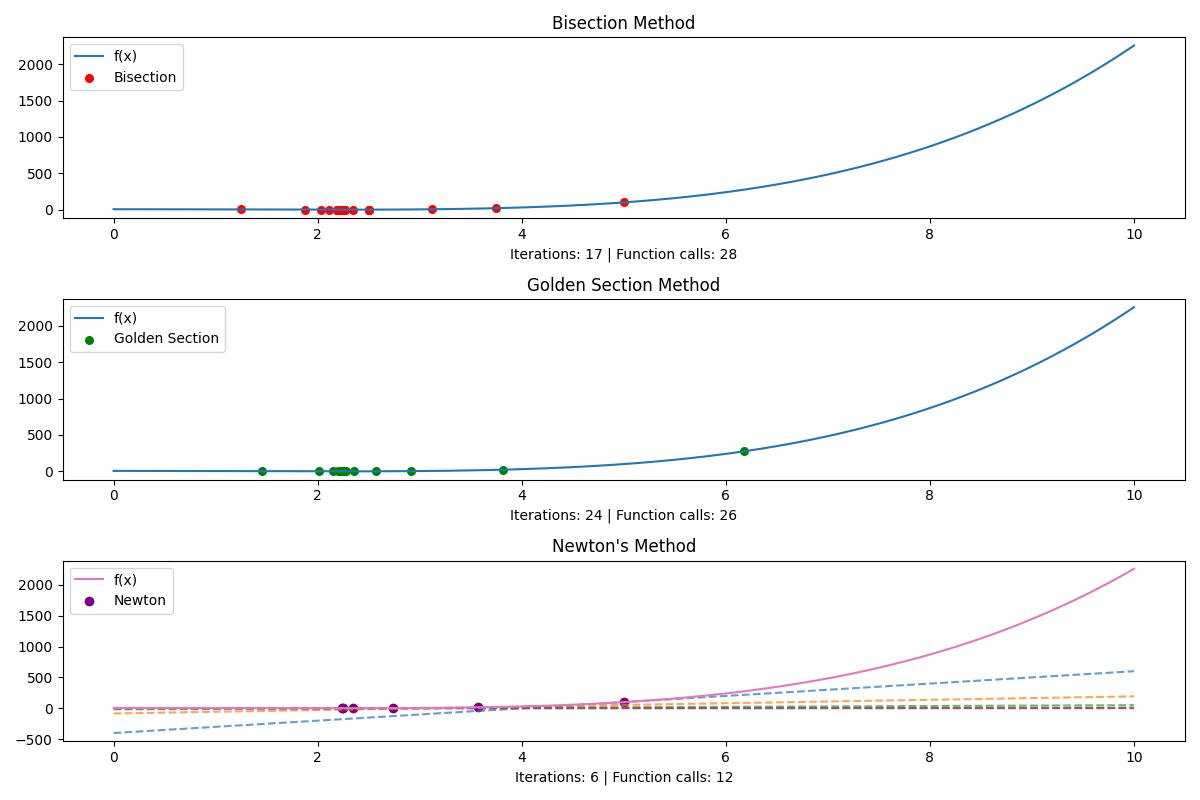
\includegraphics[width=\textwidth,height=10cm]{figure-1.jpeg}
    \caption{\label{fig:all}Funkcijos $f(x)$ optimizavimo vizualizacija.}
\end{figure}

\section{Išvados}
\begin{itemize}
    \item Visi metodai rado minimumą ties $x \approx \sqrt{5}$.
    \item Intervalo metodai (intervalo dalijimo pusiau ir auksinio pjūvio) reikalauja daugiau iteracijų ir tikslo funkcijos iškvietimų, bet yra paprastesni.
    \item Su naudotais parametrais (tikslo funkcija / intervalu / tikslumu) auksinio pjūvio optimizavimo efektyvumo pranašumas prieš intervalo dalijimo pusiau optimizavimo metodą pagal tikslo funkcijos kvietimų kiekį neišryškėjo
\end{itemize}

\section{Kodas}
\lstinputlisting[language=python]{../code/main.py}
\end{document}